\documentclass[10pt,a4paper,spanish]{article}

\usepackage[T1]{fontenc} 
\usepackage[utf8]{inputenc}
\usepackage[spanish]{babel}

\usepackage{graphicx}
\usepackage{epstopdf}

\usepackage[export]{adjustbox}
\usepackage{caption}
\usepackage{colortbl} 
\usepackage{dashrule} 
\usepackage{fancyhdr}
\usepackage{float}
\usepackage{framed}
\usepackage[bmargin=2cm,footnotesep=1cm,tmargin=2cm]{geometry} 
\usepackage[pdftex,colorlinks,backref,bookmarks=true,bookmarksnumbered=true,linkcolor=black,urlcolor=black,citecolor=black]{hyperref}
\usepackage[section]{placeins}
\usepackage[labelsep=quad,indention=10pt]{subfig}
\usepackage[spanish,shadow,textsize=small]{todonotes}
\usepackage{wrapfig}

% TITULOS
\newcommand{\asig}{Algoritmos y Estructuras de Datos}
\newcommand{\anno}{3º}
\newcommand{\grado}{Grado en Ingeniería Biomédica}
\newcommand{\upm}{Universidad Politécnica de Madrid}
\newcommand{\curso}{}
\newcommand{\ssg}{Rodrigo García Carmona}
\newcommand{\email}{\href{mailto:rodrigo.garciacarmona@ceu.es}{rodrigo.garcia@upm.es}}
\newcommand{\cabecera}[1]{
  \title{Guion de Prácticas}
  \author{\asig\\ \anno\grado\\ \ceu \\ \ssg} 
  \date{#1}
  \maketitle \thispagestyle{fancy}
}

% NUEVAS TODONOTES
\newcommand{\nota}[2][] {\todo[inline, #1]{#2}}
\newcommand{\corregir}[2][] {\todo[color=red, #1]{#2}}
\newcommand{\finaltodo}[2][] {\todo[color=green!40,fancyline #1]{#2}}
\newcommand{\finalnota}[2][] {\todo[color=green!40, inline #1]{#2}}

% PDF
\hypersetup{
  colorlinks=true,
  linkcolor=blue,
  filecolor=magenta,      
  urlcolor=cyan,
  pdfauthor={\ssg},
  pdftitle={Guion de Prácticas},
  pdfsubject={\asig, \grado, \upm, Madrid, España},
  pdfkeywords={algoritmos, estructuras de datos, ingeniería biomédica, guion, prácticas}, 
  pdftoolbar=true,
  pdfmenubar=true,
  pdffitwindow=true,
  pdfnewwindow=true
}

% ENCABEZADO
\pagestyle{fancy}%
  \renewcommand{\headrulewidth}{0.1pt}
  \renewcommand{\footrulewidth}{0.1pt}
  \fancyhf{}
  \fancyhead[L]{
\includegraphics[width=8mm]{templates/ETSIT-UPM.eps}}
  \fancyhead[C]{\small{\asig}\\\small{\grado}}
  \fancyhead[R]{\curso}
  \fancyfoot[L]{}
  \fancyfoot[C]{\thepage}
  \fancyfoot[R]{}

% CAJA SOMBREADA
% comando \sombreado{Título}{Texto}
\definecolor{shadecolor}{rgb}{0.9,0.9,0.9}
\newcommand{\sombreado}[2]{
  \begin{shaded}
    \begin{center} \emph{\textsc{#1}} \end{center}
    \noindent #2\\
  \end{shaded}
}

% CAJA INSTRUCCIONES 
\definecolor{shadecolor}{rgb}{0.9,0.9,0.9}
\newcommand{\instrucciones}[7]{
  \begin{shaded}
    \begin{center} \emph{\textsc{#1}}
    \end{center}
    %\noindent \emph{\textsc{Fecha límite de entrega: }} \emph{#4}\\
    %\emph{\textsc{Peso: }}\emph{#5}\newline\newline
    #6

    #7
  \end{shaded}
}

% Código fuente
\newcommand{\code}[1]{\texttt{#1}}

% Minted
\usepackage{minted}
% Optional: Set a default style. 'manni' is a light, clean style.
% Other popular styles include 'tango', 'monokai', 'solarized-light'.
\usemintedstyle{sas}

% PRACTICA
\newcommand{\practica}{Práctica 2: Rercursividad}
\newcommand{\notaob}{
\begin{center}
Rodrigo García Carmona\\
\href{mailto:rodrigo.garcia@upm.es}{rodrigo.garcia@upm.es}\\
\includegraphics[width=20mm]{templates/by-nc-sa.eps}
\end{center}

Esta práctica es individual y sirve tanto para desarrollar como para poner a prueba los conocimientos adquiridos. Realizar esta práctica es recomendable para aumentar las probabilidades de éxito en los exámenes teóricos.
}

% MACROS

% CONTENIDO
\begin{document}

\instrucciones{\practica}{\tiempo}{\obligatoria}{\fecha}{\peso}{\notaob}

\section{Preparación de la práctica}

El objetivo de esta práctica es interiorizar el concepto de recursividad y aprender cómo implementar métodos recursivos. Se estudiarán los siguientes conceptos:

\begin{itemize}
    \item Comprensión del concepto de recursividad.
    \item Análisis de un algoritmo recursivo.
    \item Implementación de un algoritmo recursivo.
    \item Análisis elemental del rendimiento de un programa.
\end{itemize}

\sombreado{Trabajo previo al laboratorio}{El tiempo de las clases de laboratorio es muy valioso, ya que en ellas tendrá a su disposición a los profesores para resolver cualquier duda que le pueda surgir. Por tanto, para facilitar al máximo el aprovechamiento de este tiempo, las prácticas se han dividido en varias secciones. La primera de ellas (``preparación de la práctica'') puede ¡y debe! realizarse \textbf{antes de la sesión de laboratorio} propiamente dicha. Leer esta sección antes de entrar a clase hará que su tiempo en el laboratorio sea más productivo y provocará que las dudas más importantes le surjan \textbf{durante la clase}, y \textbf{no después}, cuando se encuentre estudiando solo en su casa y la única opción que le quede sea escribir un email al profesor.

De hecho, es especialmente importante evitar que se den situaciones como esta la noche antes de un examen.}

\subsection{Exoesqueletos}

La robótica tiene numerosas aplicaciones en el campo de la ingeniería biomédica, pero para esta práctica nos centraremos en una concreta: los exoesqueletos. Estos dispositivos tienen un potencial enorme para mejorar la calidad de vida de sus usuarios, ya que pueden ayudar en un proceso de recuperación tras una lesión neurológica o servir para compensar hasta cierto punto una discapacidad. Estas aplicaciones de los exoesqueletos reciben el nombre de ``neurorehabilitación'' y ``asistencia a la discapacidad'', respectivamente:

\begin{itemize}
    \item \textbf{Neurorehabilitación:} los exoesqueletos usados en procesos de neurorrehabilitación están diseñados para ayudar a los pacientes a recuperar la función motora después de un problema neurológico, como puede ser un accidente cerebrovascular (como un ictus) o una lesión de la médula espinal. Estos dispositivos son capaces de guiar las extremidades del paciente, ayudándole a realizar el conjunto de movimientos repetitivos que conforman su terapia. La principal ventaja que ofrecen respecto a un fisioterapeuta humano es que permiten al paciente realizar la terapia durante más tiempo, con mayor consistencia y con mejor precisión. Además, los exoesqueletos también pueden registrar los datos biomecánicos del paciente durante todo el proceso, permitiendo así a los profesionales médicos monitorizar sus avances.
    \item \textbf{Asistencia a la discapacidad:} los dispositivos robóticos de asistencia a la discapacidad están diseñados para el uso diario, ayudando a las personas con discapacidades motoras a realizar actividades como caminar, levantar objetos, mantener una higiene básica o alimentarse. Estos dispositivos no buscan necesariamente ``curar'' la condición que sufre el paciente (en muchos casos, esto ni siquiera es posible), sino simplemente compensar la función perdida y dotarle de una independencia que sirva para mejorar su calidad de vida.
\end{itemize}

Un exoesqueleto robótico es una estructura externa que se coloca sobre el cuerpo de una persona. Un exoesqueleto activo (es decir, que complementa o sustituye la fuerza del paciente), tiene las siguientes partes:

\begin{itemize}
    \item Una \textbf{estructura esquelética} (el exoesqueleto propiamente dicho) que se compone de ``huesos'' o segmentos conectados mediante ``articulaciones'', y que está diseñado para poder realizar un tipo de movimientos concreto. El objetivo de esta estructura es aumentar la fuerza o restaurar la movilidad de las extremidades, y su diseño siempre está inspirado en la propia biomecánica del cuerpo humano, alineando sus articulaciones con las del usuario (cadera, rodilla, codo, etc.).
    \item Un conjunto de \textbf{motores} (también llamados ``actuadores'') que hacen posible el movimiento del exoesqueleto sin tener que recurrir únicamente a la fuerza del usuario, ya sea empleando una pequeña parte de esta o prescindiendo por completo de ella.
    \item Varios \textbf{sensores} que determinan en qué posición se encuentra cada una de las partes del exoesqueleto o miden parámetros fisiológicos del usuario.
    \item Un \textbf{sistema de control} que, a partir de la información recabada por los sensores y los objetivos terapéuticos que se desean alcanzar (moverse de determinada forma o asistir el movimiento del usuario) calcula qué órdenes concretas deben darse a los motores para que el exoesqueleto ejecute el movimiento en cuestión.
\end{itemize}

La Figura \ref{fig:hybrid-exo} ilustra cómo un exoesqueleto real (en este caso, el \href{https://www.mdpi.com/1424-8220/19/21/4773}{HYBRID}) integra todos estos componentes. En la parte izquierda de la figura puede ver la estructura esquelética e, insertada en ella, tres articulaciones para cada pierna. Una de estas articulaciones, la rodilla, aparece desglosada en la parte derecha de la figura, pudiéndose ver que está compuesta de un motor (\textit{EC60 motor}), un sensor (\textit{potentiometer}) y la electrónica necesaria para comunicarla con el sistema de control (\textit{dsPIC 30F4013}).

\begin{figure}[!htbp]
  \centering
  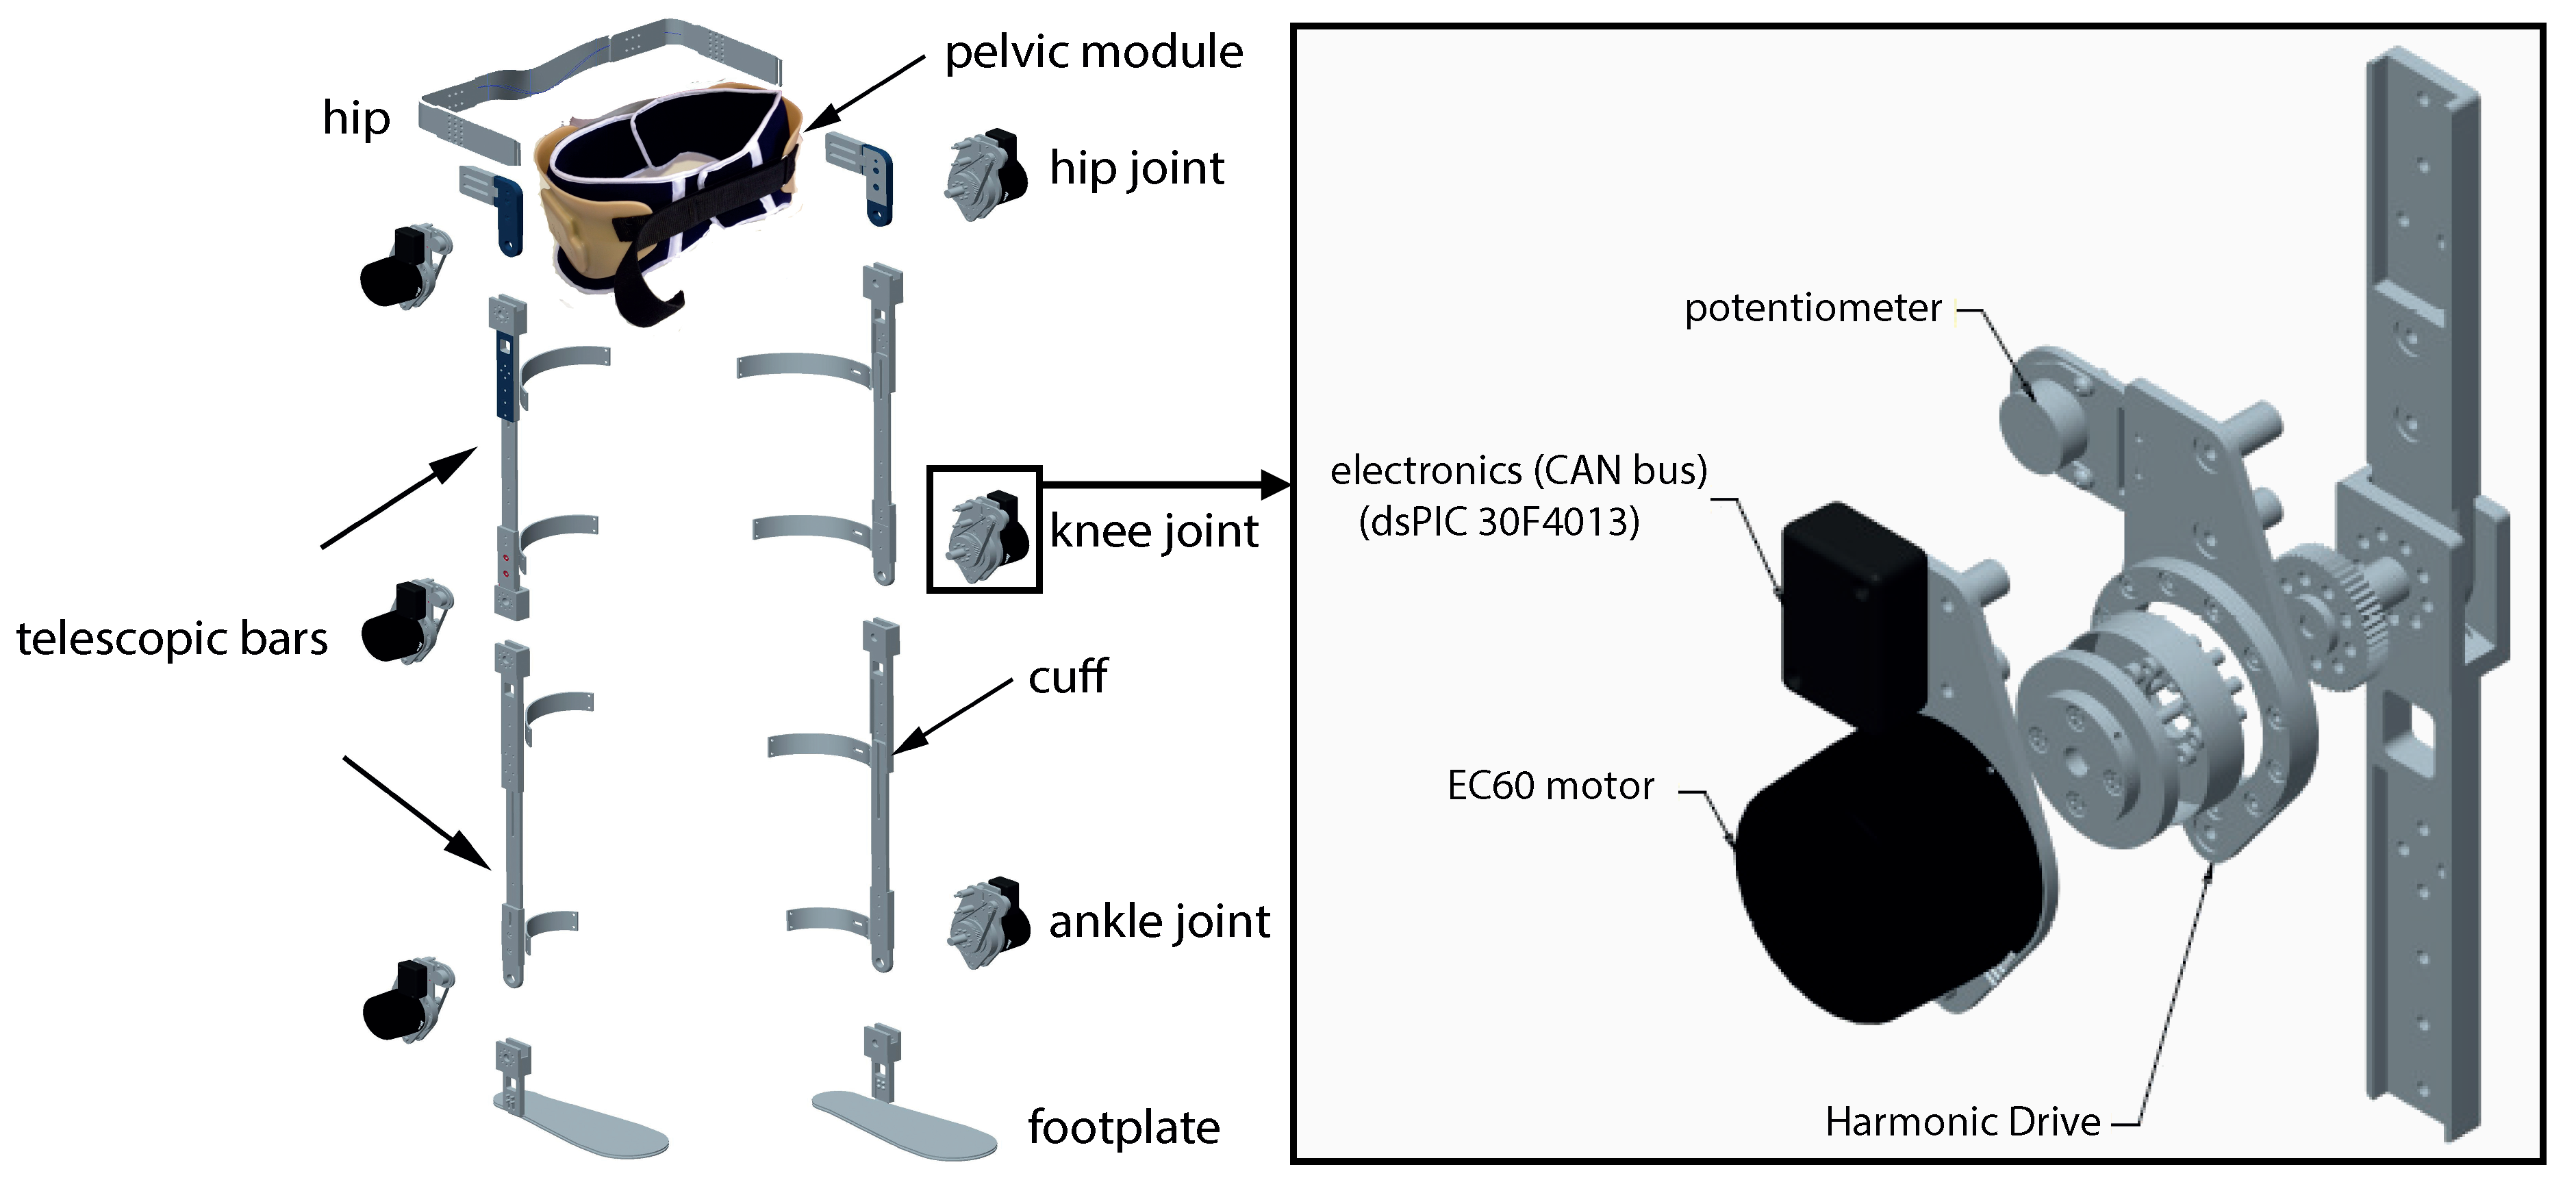
\includegraphics[width=\textwidth]{files/HYBRID-Exoskeleton.png}
  \caption[Estructura del exoesqueleto HYBRID]{Estructura del exoesqueleto HYBRID\footnotemark[1]}
  \label{fig:hybrid-exo}
\end{figure}

La Figura \ref{fig:hybrid-diagram} muestra cómo se lleva a cabo, en este mismo dispositivo, la comunicación entre las articulaciones y los sistemas de control, que se ejecutan en un pequeño ordenador (\textit{PC-104}).

\begin{figure}[!htbp]
  \centering
  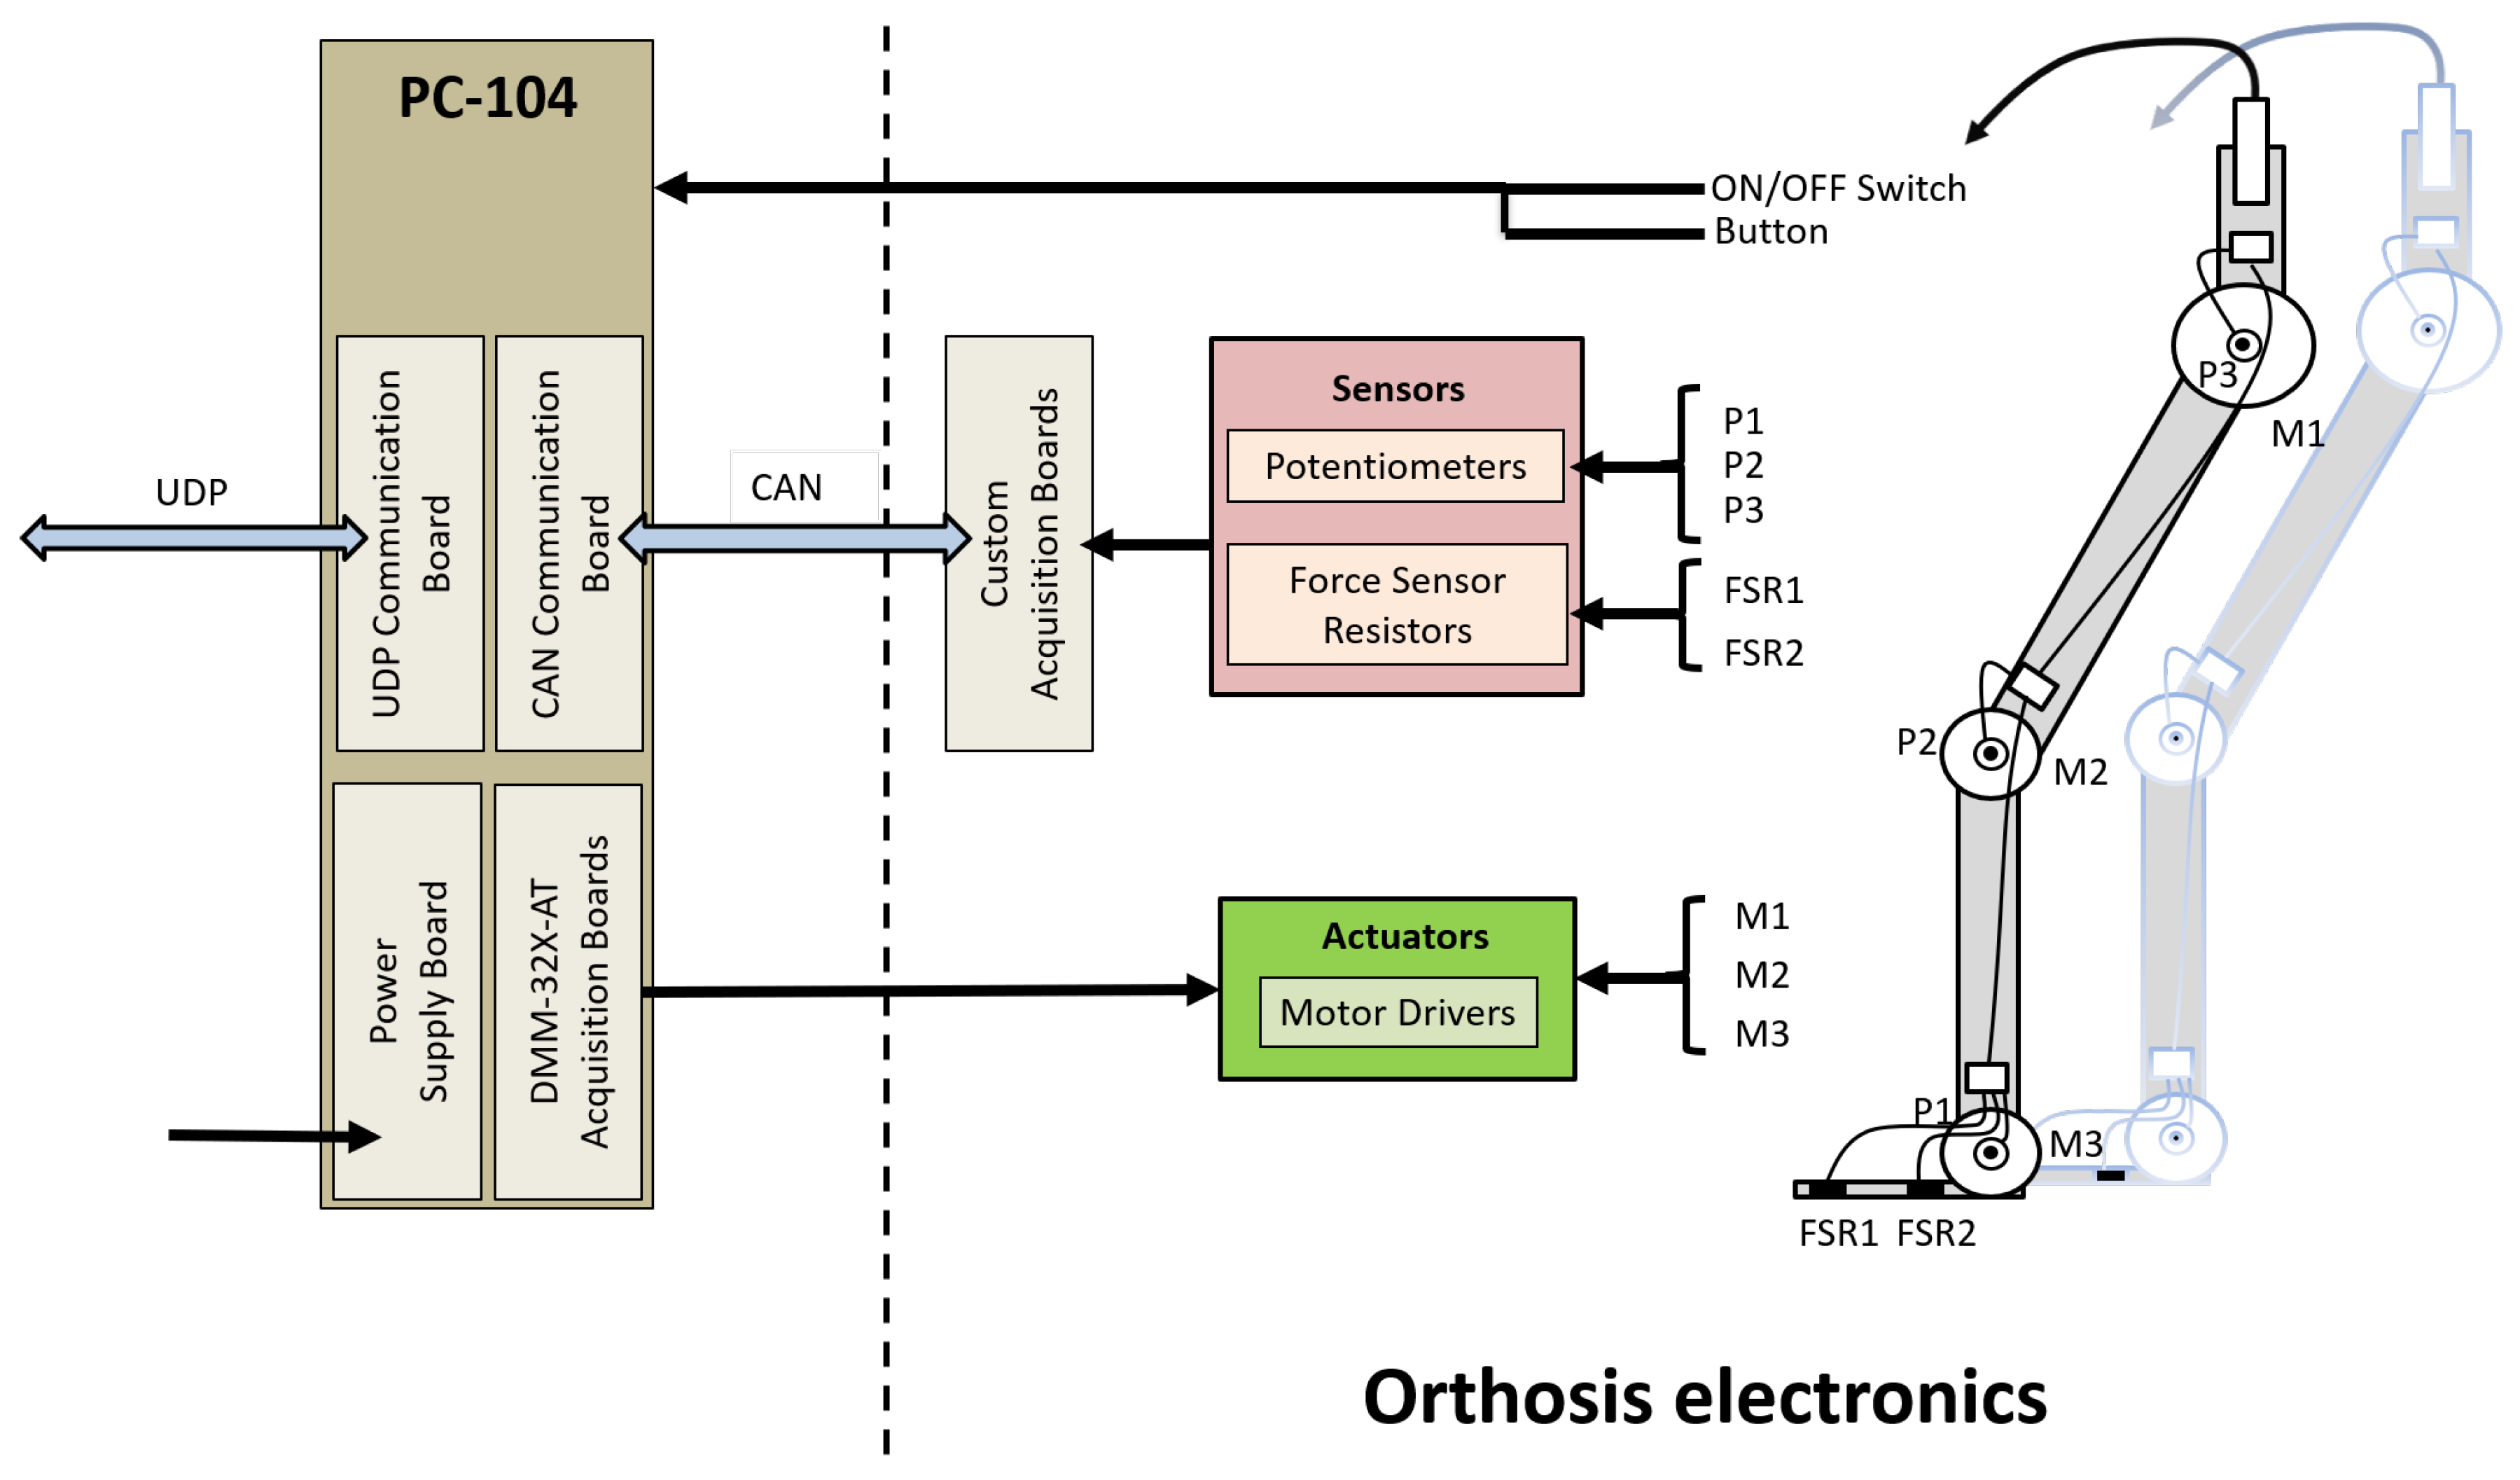
\includegraphics[width=\textwidth]{files/HYBRID-Diagram.png}
  \caption[Conexión del exoeskeleto HYBRID con su sistema de control]{Conexión del exoeskeleto HYBRID con su sistema de control\footnotemark[1]}
  \label{fig:hybrid-diagram}
\end{figure}
\footnotetext[1]{\href{https://www.mdpi.com/1424-8220/19/21/4773}{Eloy Urendes, Guillermo Asín-Prieto, Ramón Ceres, Rodrigo García-Carmona, Rafael Raya y José L. Pons.}}

\sombreado{Prótesis robóticas}{Las prótesis, es decir, la sustitución de un miembro perdido por uno artificial, han existido desde hace siglos, pero gracias a la robótica es posible construir prótesis ``biónicas'', que utilizan motores, microprocesadores y componentes electrónicos para imitar de forma mucho más fiel la funcionalidad de la extremidad perdida.

De hecho, no hay mucha diferencia desde un punto de vista ingenieril entre el desarrollo de una prótesis o de un exoesqueleto: ambos son dispositivos robóticos que utilizan sensores, motores y un sistema de control para ejecutar un movimiento concreto. La diferencia fundamental es que los exoesqueletos se sitúan sobre el cuerpo humano y las prótesis sustituyen alguna parte del mismo.}

El funcionamiento de un exoesqueleto exige un control sumamente preciso, pues estamos trabajando con motores capaces de ejercer una gran fuerza, suficiente para hacer daño al paciente si le obligan a asumir una postura incorrecta. Y aquí es donde entra en juego el sistema de control del que se hablaba antes. Este sistema es el cerebro del exoesqueleto, el responsable de decidir cómo deben moverse los motores siguiendo un algoritmo programado en \textit{software}.

\subsection{Cinemática directa}

Uno de los problemas más comunes que el \textit{software} del sistema de control de un exoesqueleto debe resolver es el de la cinemática directa (\textit{forward kinematics} en inglés). Este proceso consiste en calcular la \textbf{posición y orientación} del extremo final del exoesqueleto (llamado en inglés \textit{end-effector}) a partir de las \textbf{carácterísticas de sus segmentos} (los ``huesos'') y los \textbf{ángulos} que estos forman.

\sombreado{Cinemática}{Recordará, de sus clases de física, que la cinemática es la rama de la mecánica que describe el movimiento de los objetos sin tener en cuenta las fuerzas que lo causan. Por tanto, en esta práctica lo único que tendremos en cuenta será la posición en el espacio de cada una de las partes del exoesqueleto.}

Imaginemos el exoesqueleto de un brazo, compuesto por una \textbf{cadena} de varios segmentos: un brazo, un antebrazo y una mano, en la que el brazo está conectado con el antebrazo, y el antebrazo a su vez con la mano. Si conocemos:

\begin{itemize}
    \item los parámetros geométricos de cada uno de los segmentos,
    \item el ángulo que forman con el segmento anterior de la cadena, y
    \item la posición y orientación absolutas del primer segmento de la cadena,
\end{itemize}

la cinemática directa nos proporciona un conjunto de ecuaciones con las que calcular la ubicación precisa del extremo final de la mano en un sistema de coordenadas tridimensional $(x, y, z)$, así como su orientación $(\alpha, \beta, \gamma)$.

\sombreado{Orientación y sistemas de coordenadas}{Los tres ángulos de la orientación reciben diferentes denominaciones en el mundo de la computación y en el de la medicina. En el de la computación se conocen como ``balanceo'', ``cabeceo'' y ``guiñada'', términos heredados de la aeronáutica. En el de la medicina se trabaja con los ángulos de los planos anatómicos, siendo estos el ``sagital'', el ``frontal'' y el ``transversal''.

Para complicar aún más este asunto, hay que tener en cuenta que los sistemas de coordenadas tridimensionales pueden seguir la regla de la mano izquierda o la de la mano derecha. Si siente curiosidad, investigue todo esto.}

El control de movimientos es la aplicación más directa de la cinemática directa. Por ejemplo: para que un exoesqueleto guíe la pierna de un paciente a través de una trayectoria de marcha específica, el sistema de control debe recurrir constantemente a la cinemática directa para verificar que la posición del pie del exoesqueleto coincide con la posición deseada en cada instante. Si detecta un error, deberá ajustar los motores de las articulaciones para corregirlo.

De hecho, este proceso puede realizarse antes de ejecutar el movimiento, verificando así que este no hará que el exoesqueleto colisione consigo mismo o con el entorno. También permite definir un espacio de trabajo seguro que el exoesqueleto no deberá abandonar bajo ningún concepto, para así proteger al usuario y a los que le rodean. Recuerde que un exoesqueleto puede ejercer mucha fuerza.

En esencia, la cinemática directa es el puente entre los comandos enviados por el sistema de control a los motores (los ángulos de las articulaciones) y el comportamiento resultante del dispositivo en el mundo real. Sin ella, sería imposible lograr un control preciso y seguro en la robótica biomédica.

\subsection{Resolución del problema de la cinemática directa en 3 dimensiones}

El método más común para resolver el problema de la cinemática directa emplea \textbf{matrices de transformación homogénea}, que describen la relación espacial entre un segmento de la cadena y el siguiente.

Una matriz de transformación homogénea es una matriz $4\times4$ que puede representar tanto la rotación como la traslación de un marco de referencia con respecto a otro en una sola operación. Para un exoesqueleto con $n$ segmentos, la posición y orientación del extremo final con respecto al primer segmento se calcula multiplicando las matrices de transformación de cada segmento en secuencia:

$$T_{final} = T_1 \cdot T_2 \cdot T_3 \cdot \ldots \cdot T_n$$

Donde cada matriz $T_i$ depende del ángulo del segmento $\theta_i$ y de sus características geométricas (como su longitud o su forma). El resultado, $T_{final}$, es una matriz que contiene las coordenadas $(x, y, z)$ de la posición del extremo final y los datos que definen su orientación. Una de las convenciones más utilizadas para definir estas matrices es la de Denavit-Hartenberg, pero no es la única.

Si, llegados a este punto, está asustado (el álgebra suele producir este efecto en los estudiantes), no se preocupe: para la práctica utilizaremos un modelo de cinemática inversa más sencillo, en 2 dimensiones, por lo que los cálculos serán más sencillos.

\subsection{Resolución del problema de la cinemática directa en 2 dimensiones}
\label{sec:problema2d}

Consideraremos una versión simplificada del modelo de cinemática directa, en el que solo se trabaja con dos coordenadas $(x, y)$, y los segmentos son siempre rectos y tienen una longitud fija.

De cada segmento conocemos:

\begin{itemize}
    \item La \textbf{longitud} del segmento.
    \item El \textbf{ángulo} que forma con su segmento padre (al que está conectado).
    \item Sus \textbf{segmentos hijos} (los que están conectados a él).
\end{itemize}

\sombreado{Varios hijos}{\textbf{Importante:} Recuerde que cada segmento puede tener varios hijos. Piense cómo el segmento que representa su muñeca está unido a cinco segmentos que representan los metacarpos de cada dedo.}

Además, también conocemos la posición $(x,y)$ del \textbf{punto inicial} del \textbf{segmento raíz}: el único segmento que no tiene un segmento padre.

Para calcular la posición $(x,y)$ del \textbf{punto final} de un segmento concreto ($s_i$) se utilizarán la siguientes ecuaciones, obtenidas mediante trigonometría:

$$x_i = x_{i-1} + L_i \cos{(\theta_1 + \cdots + \theta_i)} $$
$$y_i = y_{i-1} + L_i \sin{(\theta_1 + \cdots + \theta_i)} $$

En las que $x_{i-1}$ e $y_{i-1}$ son la posición del punto final del segmento padre (o, si se trata del segmento raíz, de su punto inicial, pues no tiene padre), y $\theta$ son los ángulos de la cadena de segmentos que conducen desde el segmento raíz hasta el segmento actual (inclusive). Si, por ejemplo, el segmento que deseamos calcular ($s_3$) está conectado de la siguiente forma: $s_3 \to s_2 \to s_1$ y $s_1$ es el segmento raíz:

\begin{itemize}
    \item $\theta_1$: Ángulo del segmento raíz ($s_1$).
    \item $\theta_2$: Ángulo del segmento ($s_2$) conectado al segmento raíz ($s_1$).
    \item $\theta_3$: Ángulo del segmento ($s_3$) conectado al segmento ($s_2$) conectado al segmento raíz ($s_1$).
\end{itemize}

Las ecuaciones quedarían:

$$x_3 = x_{2} + L_3 \cos{(\theta_1 + \theta_2 + \theta_3)} $$
$$y_3 = y_{2} + L_3 \sin{(\theta_1 + \theta_2 + \theta_3)} $$

Para comprobar que ha entendido cómo resolver este problema, \textbf{realice, de forma manual (sin programarlo), el siguiente ejercicio:} Considere una cadena cinemática compuesta de los siguientes segmentos:

\begin{itemize}
    \item \textbf{Segmento 1 (raíz):} En la posición $(0,0)$, de longitud 4, formado un ángulo de 45\textdegree.
    \item \textbf{Segmento 2:} Hijo del segmento 1, de longitud 2, formando un ángulo de 45\textdegree.
    \item \textbf{Segmento 3:} Hijo del segmento 2, de longitud 1, formando un ángulo de 90\textdegree.
    \item \textbf{Segmento 4:} Hijo del segmento 2 (¡sí, del 2!), de longitud 1, formando un ángulo de \textminus90\textdegree.
\end{itemize}

\textbf{¿Cuál es la posición del extremo final de los segmentos 3 y 4?}

\vspace{1cm}

¡No pase a la página siguiente hasta haber terminado! ¡No haga trampas!

\vspace{1cm}

...

\vspace{1cm}

Si ha hecho bien los cálculos, deberían haber obtenido el siguiente resultado:

$$(x_3,y_3) = (2\sqrt{2}-1, 2\sqrt{2}+2)$$
$$(x_4,y_4) = (2\sqrt{2}+1, 2\sqrt{2}+2)$$

\sombreado{Recursividad}{Alguien de mente astuta como usted sin duda habrá sospechado que el problema de la cinemática directa tiene algo que ver con la recursividad, pues para eso forma parte de esta práctica. Repase los cálculos que ha hecho para resolver el ejercicio (porque lo ha resuelto, ¿verdad?) y fíjese en que para poder calcular la posición de un segmento primero es necesario haber calculado la de su padre. Y, para la calcular la posición del segmento padre, será necesario calcular la del ``abuelo'', y así sucesivamente...

Efectivamente, una cadena cinemática es una estructura que se presta de forma natural a la recursividad. La dependencia secuencial entre segmentos es inherentemente recursiva. Además, un algoritmo recursivo podrá calcular la cinemática directa para un número arbitrariamente grande de segmentos. En lo que a la implementación del algoritmo respecta, tanto da que nuestro exoesqueleto tenga 3 como 300 segmentos.}

\subsection{Objetivo y descarga de la práctica}

El objetivo de la práctica es terminar de desarrollar una aplicación Java que permite visualizar la posición de los segmentos de un exoesqueleto en un espacio bidimensional. Además, esta aplicación también muestra el movimiento de dicho exoesqueleto de forma animada, permitiendo cargar la secuencia de movimientos desde un archivo.

La práctica está disponible en GitHub, en la siguiente dirección de Internet (URI):

\href{https://github.com/rgarciacarmona/ALED-lab2}{https://github.com/rgarciacarmona/ALED-lab2}

Recuerde que, para poder importar el repositorio en Eclipse debe seleccionar \textit{File $\to$ Import...} y, de entre las opciones disponibles, \textit{Git $\to$ Projects from Git $\to$ Clone URI}. A continuación le aparecerá un menú en el que tendrá que introducir la URI que aparece en el párrafo anterior.

Tómese su tiempo para examinar todas las clases del proyecto que acaba de importar. Intente figurarse, a base de observar el código, para qué sirve cada una de ellas.

\subsection{Modelado de datos}

A la hora de resolver un problema (ya sea biomédico o de cualquier otro ámbito) programando, el primer paso será modelar los datos con los que vamos a tener que trabajar. Dicho de otra forma: tenemos que pensar cómo podemos representar la información que es importante para nosotros en un formato que el ordenador entienda.

En lo que a esta práctica respecta, los segmentos estarán representados mediante la clase \code{Segment} del paquete \code{es.upm.aled.lab2.kinematics}, que está sin implementar. Esta clase deberá contener toda la información de la que disponemos \textbf{para cada segmento}. A saber:

\begin{itemize}
    \item La \textbf{longitud} del segmento, en cm. La modelaremos mediante un \code{double} al que llamaremos \code{length}.
    \item El \textbf{ángulo} que forma con su segmento padre, en radianes. Lo modelaremos usando un \code{double} al que llamaremos \code{angle}.
    \item Sus \textbf{segmentos hijos}. Los modelaremos como usando una \code{List<Segment>} a la que llamaremos \code{children}.
\end{itemize}

No será necesario almacenar la posición del punto inicial del segmento raíz. Asumiremos que será el origen de coordenadas o, en caso contrario, que nos la proporcionará quien use la clase.

Además, la aplicación cuenta con una interfaz gráfica que permitirá representar los segmentos en forma de un esqueleto capaz de animarse. Este esqueleto está formado por nodos: objetos de la clase \code{Node} del paquete \code{es.upm.aled.lab2.gui}.

\code{Node} tiene los siguientes atributos:

\begin{itemize}
    \item \code{double x} y \code{double y}: las coordenadas del nodo. El programa dibujará un punto aquí.
    \item \code{List<Node> children}: los nodos conectados con este. El programa dibujará una línea desde las coordenadas de este nodo hasta cada uno de los nodos a los que esté conectados..
\end{itemize}

La Figura \ref{fig:uml} muestra ambas clases.

\begin{figure}[!htbp]
  \centering
  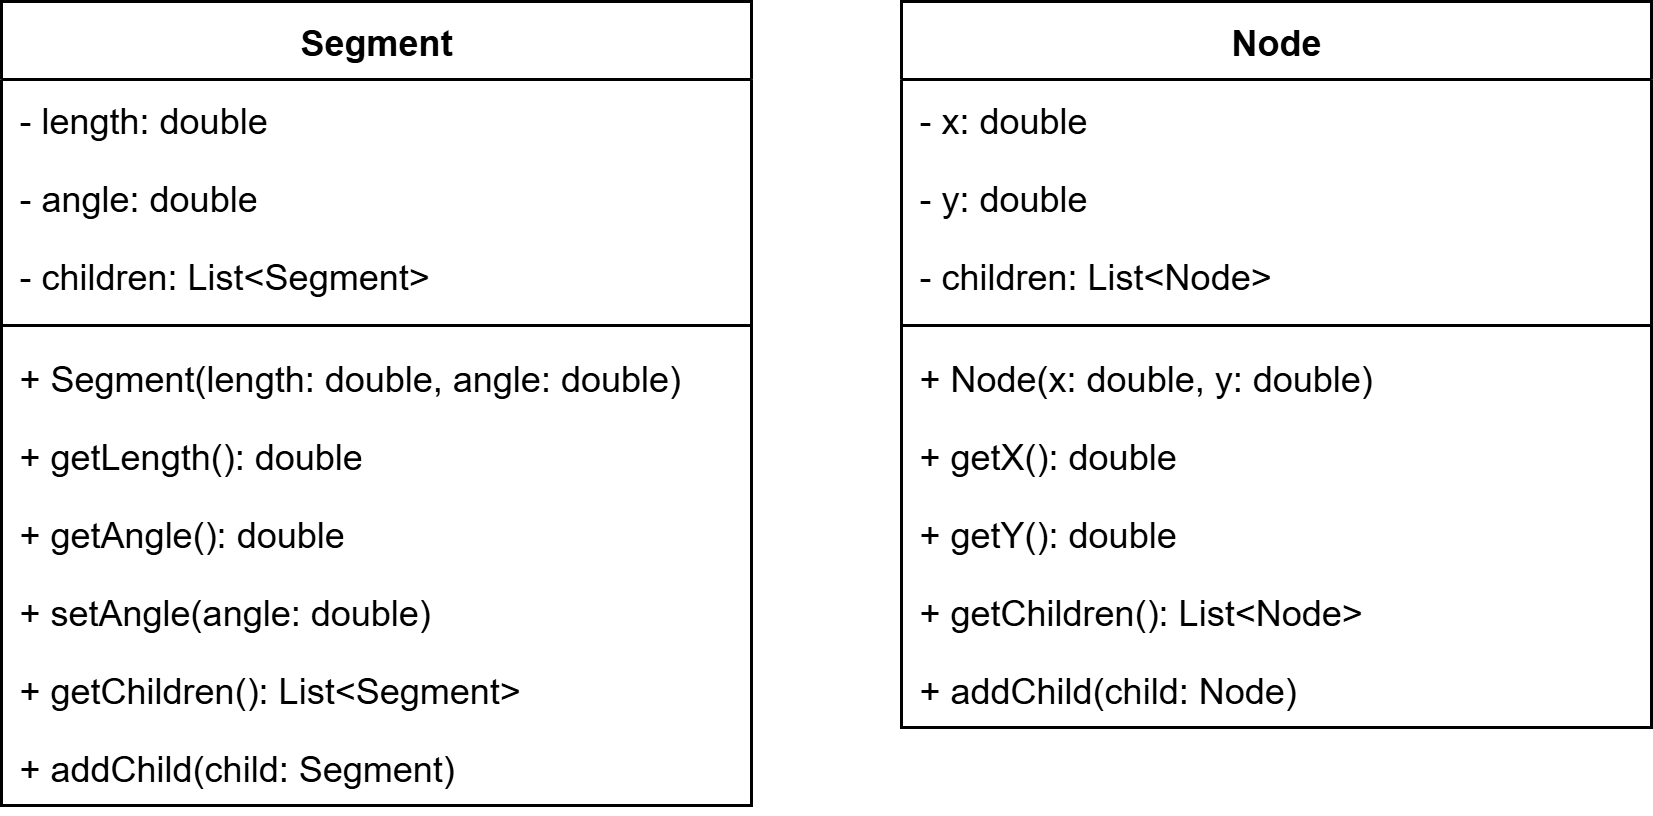
\includegraphics[width=0.8\textwidth]{files/ALED-2-DataModel.png}
  \caption{Diagrama de clases del modelo de datos de la práctica}
  \label{fig:uml}
\end{figure}

\textbf{Responda a las siguientes preguntas:}

\begin{itemize}
    \item ¿Tienen \code{Segment} y \code{Node} métodos \textit{getters}? ¿Cuáles son?
    \item ¿Tienen \code{Segment} y \code{Node} métodos \textit{setters}? ¿Cuáles son?
    \item ¿Son \code{Segment} y \code{Node} tipos de datos recursivos?
\end{itemize}

Enhorabuena, ya ha terminado con el trabajo previo a la sesión de laboratorio. Las secciones de la \ref{sec:laboratorio} en adelante puede realizarlas en clase.

\section{Implementación de la clase \code{Segment}}
\label{sec:laboratorio}

En primer lugar, programará la clase \code{Segment} del paquete \code{es.upm.aled.lab2.kinematics}, que ya está creada pero que se encuentra vacía. Esto le permitirá interiorizar la estructura de esta clase, que tendrá que manejar posteriormente (en la sección \ref{sec:recursividadImpl}), cuando tenga que implementar un algoritmo recursivo usándola.

\subsection{Implementación de los métodos y atributos}
\label{sec:implSegment}

Observe la Figura \ref{fig:uml}, y fíjese en los métodos y los atributos de la clase \code{Segment}. Impleméntelos. En cada caso, el nombre del método deberá ser lo bastante autoexplicativo como para que pueda deducir qué debe hacer cada uno. No obstante, en el caso de uno de los métodos ( \code{addChild()}() hay un aspecto importante que debe tener en cuenta y que no resulta obvio se deduce inmediatamente a partir del nombre: no debe añadirse un nuevo \code{Segment} a la lista de hijos si este ya se encontraba en ella. De no hacerse esta comprobación, podríamos acabar con una cadena cinemática con elementos duplicados.

Si no sabe por dónde empezar, estudie el funcionamiento de la clase \code{Node}, que se encuentra en el paquete \code{es.upm.aled.lab2.gui}, ya que es similar en muchos aspectos a la que tiene que implementar usted.

\subsection{Documentación del código}

Ahora que ha terminado de programar la clase \code{Segment}, es hora de documentarla. Añada todos los comentarios que considere necesarios. En caso de duda, siempre es mejor pasarse que quedarse corto.

Y sí, hemos dicho antes que el nombre de los métodos debería ser autoexplicativo a la hora de comunicar qué hacen, pero asuma que quién está leyendo su código no es tan listo como usted (o, si lo es, que ha pasado una mala noche). De nuevo, para ver cómo se documenta bien una clase, puede inspirarse en cómo se ha hecho esto en \code{Node}.

\section{Análisis de un algoritmo recursivo}

Antes de que programe usted mismo un algoritmo recursivo, va a analizar uno que ya está implementado: el que se utiliza para dibujar los \code{Nodes} en pantalla. Abra la clase \code{SkeletonPanel}, que se encuentra en el paquete \code{es.upm.aled.lab2.gui}, y dedique un tiempo a leerla e intentar entender lo que hace. Este proceso le hará ser consciente de lo importantes que son los comentarios, si es que no estaba convencido aún de ello.

\textbf{Responda a las siguientes preguntas:}

\begin{itemize}
    \item ¿Qué tareas realiza el constructor?
    \item ¿Qué hace el método \code{paintComponent()}?
    \item ¿A qué dos métodos, que representan cada uno un algoritmo recursivo distinto, llama el método \code{paintComponent()}? ¿Cuál de ellos ya está implementado?
    \item ¿Alguno de los métodos de \code{SkeletonPanel} se llama a sí mismo?
\end{itemize}

\subsection{Documentación del código}

Llegados a este punto, ya se habrá dado cuenta de que el método \code{drawSkeleton()} contiene la implementación de un algoritmo recursivo: el que pinta en pantalla cada uno de los \code{Nodes} de los que se compone el dibujo de un exoesqueleto. Puede haberse percatado de esto siguiendo uno de los tres acercamientos siguientes:

\begin{enumerate}
    \item Ha razonado que todos los \code{Nodes} están conectados con, al menos, otro. Eso significa que, para poder dibujar la línea que llega hasta un \code{Node} nuevo será necesario haber dibujado primero el otro \code{Node} (exceptuando el primer \code{Node}, cuya línea va al origen).
    \item Ha intuido que los \code{Nodes} están relacionados siguiendo una estructura de árbol, por lo que si se quiere obtener la información de un \code{Node} concreto es preciso llamar al método \code{getChildren()} de su padre. Pero claro, para obtener la información de este padre, primero será necesario haber llamar al método \code{getChildren()} del ``abuelo'', y así sucesivamente, repitiendo este proceso tantas veces como sea necesario.
    \item Ha leído el código y se ha dado cuenta de que \code{drawSkeleton()} llama a \code{drawSkeleton()} (posiblemente más de una vez, pues lo hace dentro de un \code{for}), pasándole unos parámetros distintos a lo que recibió. Esto significa que cada \code{drawSkeleton()} solo retornará cuando lo hayan hecho todos los \code{drawSkeleton()} a los que este ha llamado.
\end{enumerate}

\sombreado{Diferentes formas de pensar}{No importa cuál de las líneas de razonamiento haya seguido para llegar a la conclusión de que \code{drawSkeleton()} implementa un algoritmo recursivo. Cada persona tiene una manera de razonar que le resulta más intuitiva que el resto, por lo que suele recurrir a ella para llegar a las conclusiones correctas lo más fácilmente posible. Quizá usted tenga un pensamiento más ``algorítmico'' y haya razonado como se indica en el acercamiento 3, o quizá prefiera visualizar las cosas y por eso haya seguido el 2. En cualquier caso, no importa; bien está lo que bien acaba.

Eso sí, si puede, intente entender el porqué de los razonamientos que no ha seguido, para ir ejercitando su mente y acostumbrándose a pensar en diferentes formas de idear soluciones a problemas reales.}

\textbf{Responda a las siguientes preguntas:}

\begin{itemize}
    \item ¿Qué líneas de código representan el caso base?
    \item ¿Qué líneas de código representan el paso recursivo?
    \item ¿Qué líneas de código representan el código general o común?
    \item ¿Qué se dibuja primero, el final (extremo final del último segmento) o el principio (punto inicial del segmento raíz) de la cadena cinemática? Le recomiendo recurrir al depurador para confirmar si su respuesta es correcta o no.
\end{itemize}

Por último, ahora que sabe para qué sirve cada una de las líneas de código de \code{drawSkeleton()}, añada tantos comentarios como sea necesario (de nuevo, cuantos más mejor) al interior de este método, para que quede claro cómo funciona.

\section{Implementación de un algoritmo recursivo}
\label{sec:recursividadImpl}

Ahora que ya ha analizado un algoritmo recursivo, ha llegado el momento de que implemente el suyo propio. Cuando analizó el método \code{drawSkeleton()} de la clase \code{SkeletonPanel}, observó que llamaba al método \code{computePositions()} de la clase \code{ForwardKinematics}. Abra ahora esta clase, porque tendrá que implementar los dos métodos que contiene.

Antes de continuar leyendo, repase el procedimiento para la resolución del problema de la cinemática directa en 2 dimensiones que aparecía en la sección \ref{sec:problema2d}. Lo que hará a continuación será precisamente implementar dicho algoritmo.

\subsection{Implementar el método fachada}

En muchas implementaciones de algoritmos recursivos, el método al que se llama recursivamente necesita una serie de argumentos ``adicionales'', que van cambiando en cada llamada a dicho método pero que el usuario que inicia el algoritmo no tiene que proporcionar.

En problemas en los que se da esta circunstancia, es habitual separar la implementación en:

\begin{itemize}
    \item Un \textbf{método recursivo} privado, que es la implementación del algoritmo recursivo propiamente dicho.
    \item Un \textbf{método fachada} público, al que llama el que invoca el algoritmo recursivo. Este método fachada hace la primera llamada al método recursivo.
\end{itemize}

En el ejemplo que nos ocupa, el método fachada recibe como argumentos:

\begin{itemize}
    \item \code{root}: El \code{Segment} raíz del árbol de segmentos.
    \item \code{originX} y \code{originY}: Las coordenadas del punto inicial del segmento raíz.
\end{itemize}

Mientras que el método privado recibe, además de estos argumentos, un \code{accumulatedAngle}, que se va incrementando según se va avanzando por el árbol de segmentos. De nuevo, revise las ecuaciones de la sección \ref{sec:problema2d} para entender por qué el ángulo se va acumulando.

Implemente el método fachada, que deberá llamar al método privado pasándole los mismos argumentos que ha recibido y un \code{accumulatedAngle} de 0, ya que al principio del algoritmo no hay ningún ángulo previo que sumar al actual.

\subsection{Implementar el método privado}

Ahora implemente el auténtico algoritmo recursivodentro del método privado. Este apartado le llevará la mayor parte del trabajo de esta práctica, así que dedíquele todo el tiempo que sea necesario, no se frustre, y recurra tanto al papel como al depurador cuantas veces sea necesario.

Para resolver con éxito esta parte de la práctica, tenga en cuenta lo siguiente:

\begin{itemize}
    \item El método que está implementando devuelve un \code{Node}, no un \code{Segment} (\code{Segment} es lo que recibe como argumento).
    \item El método que está implementando devuelve un \code{Node}. Esto significa que no es necesario devolver una \code{List<Node>} o ninguna otra colección similar, porque cada \code{Node} ya contiene una \code{List} con sus hijos.
    \item Hablando de lo cual... No olvide añadir cada \code{Node} a la lista de hijos de su \code{Node} padre después de haber calculado su posición. El único \code{Node} que no tendrá hijos será el último de cada rama del árbol.
    \item Uno de los aspectos más importantes a la hora de implementar un algoritmo usando recursividad es el caso base. Para este problema, el caso base deberá ocurrir cuando el \code{Segment} que se pasa al método recursivo no tenga hijos. Si se da esta circunstancia, deberá construirse el \code{Node} pertinente, pero este no tendrá tampoco hijos.
    \item En el paso recursivo, ponga cuidado en que los argumentos que se pasa a la nueva llamada al método son los correctos. Un error muy común es pasar otra vez los argumentos que ya se habían recibido de la anterior llamada.
    \item Piense en qué aspectos del algoritmo pueden considerarse código general. Serán siempre aquellos cálculos que sea necesario realizar en todas las llamadas, tanto si estamos hablando del caso base como de los pasos recursivos intermedios.
\end{itemize}

\subsection{Ejecutar el método \textit{main}}

Para comprobar que el código que ha escrito funciona, se ha preparado una clase \code{SkeletonVisualizer}, cuyo método \code{main} lleva a cabo las siguientes tareas:

\begin{enumerate}
    \item Construye una cadena cinemática que representa un exoesqueleto de cuerpo entero con 10 segmentos: torso, cuello, brazo izquierdo, antebrazo izquierdo, brazo derecho, antebrazo derecho, muslo izquierdo, pantorrilla izquierda, muslo derecho y pantorrilla derecha.
    \item Abre una ventana y representa gráficamente este exoesqueleto.
    \item Si se le pasa un argumento al método \code{main}, abrirá el archivo cuya ubicación coincida con este argumento. Dicho archivo deberá está formateado en CSV (como en la práctica 1) y contener una secuencia de movimientos \textit{frame} a \textit{frame} para 8 de las extremidades de este exoesqueleto. Junto con la práctica se le proporciona un archivo con una secuencia de movimientos de ejemplo, llamado \textit{walking\_cycle.csv}, que se encuentra en la carpeta \textit{animations}.
    \item Si ha conseguido cargar el contenido de un archivo, el programa anima el exoesqueleto en un bucle de rebote (primero en un sentido, luego en otro, luego de vuelta al sentido original, y así \textit{ad infinitum}) a partir de los datos de movimiento recibidos.
\end{enumerate}

Utilice este \code{main} para poner a prueba el código que ha escrito. Si ha implementado correctamente el algoritmo recursivo, debería ver una ventana como la de la Figura \ref{fig:sampleExoskeleton}. Si no, es que ha hecho algo mal y habrá llegado el momento de depurar.

\begin{figure}[!htbp]
  \centering
  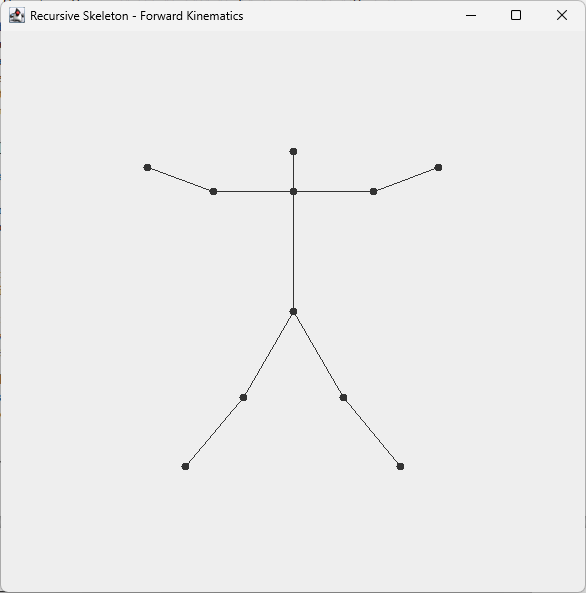
\includegraphics[width=0.62\textwidth]{files/Exoskeleton-Drawing.png}
  \caption{Dibujo del exoesqueleto de ejemplo}
  \label{fig:sampleExoskeleton}
\end{figure}

Recuerde que, por defecto, al ejecutar el método \code{main} de una clase, Eclipse no le pasa ningún argumento. Por tanto, si hace una ejecución directa el programa simplemente representará el exoesqueleto de forma estática, sin animarlo. Por tanto, si quiere que su exoesqueleto se mueva (se lo recomiendo, la verdad es que resulta gracioso), tendrá que crear una configuración de lanzamiento, como ya hizo en la práctica 1.

\textbf{Responda a las siguientes preguntas:}

\begin{itemize}
    \item ¿Cómo debe modificar el código del \code{main} para que los segmentos sean más largos o más cortos?
    \item ¿Cómo debe modificar el código del \code{main} para añadir tres dedos a cada mano?
\end{itemize}

\section{Medida de tiempos}

Más adelante, en esta asignatura, verá lo importante que es analizar el rendimiento de un algoritmo. Para ir abriéndole el apetito, instrumentalizará (de forma bastante inocente) su código, de tal manera que pueda observar el tiempo que lleva la ejecución de cada invocación del método \code{computePositions()} (la versión privada, no la fachada) que usted mismo ha programado.

La forma de hacer esto será anotar el instante de tiempo en el que comienza el método y el instante de tiempo en el que termina y restar ambos valores. El resultado será el tiempo que ha tardado el método en ejecutarse. En Java, puede obtener el instante de tiempo en nanosegundos en el que ocurre algo mediante el método estático \code{nanoTime()} de la clase \code{System}.

Por tanto, escriba el siguiente código al principio del cuerpo del método \code{computePositions()}:

\begin{minted}[
  frame=lines, % Adds a frame around the code
  framesep=2mm,
  % linenos % Enables line numbers
]{java}
long startTime = System.nanoTime();
\end{minted}

Y el siguiente código al final, justo antes del \code{return} (¡tenga en cuenta que puede haber varios \code{return}!):

\begin{minted}[
  frame=lines, % Adds a frame around the code
  framesep=2mm,
  % linenos % Enables line numbers
]{java}
long runningTime = System.nanoTime() - startTime;
System.out.println("Tiempo de computePositions para un segmento con "
                   + link.getChildren().size() + " hijos: "
                   + runningTime + " nanosegundos");
\end{minted}

Después, ejecute el código y fíjese en lo que aparece en el terminal.

\textbf{Responda a las siguientes preguntas:}

\begin{itemize}
    \item ¿Cómo varía el tiempo de ejecución en función del número de hijos del \code{Segment}?
    \item ¿Tiene alguna teoría de por qué ocurre esto?
\end{itemize}

Si siente curiosidad, instrumentalice otras partes de su código. Enhorabuena, ha terminado la práctica.

\section{Extras}

Si siente curiosidad, pruebe a llevar a cabo las tareas siguientes:

\begin{itemize}
    \item Averigüe lo que significa el \code{@Override} que aparece encima de \code{paintComponent()} en la clase \code{SkeletonPanel}.
    \item Averigüe lo que significa el operador \code{->} en Java. Aparece en el \code{main}, en la línea en la que se crea el \code{Timer} que controla la animación.
    \item Cree su propio archivo de secuencia de movimientos, que ejecute algún movimiento curioso como mover un solo brazo, hacer un saludo militar o dar saltitos.
    \item Modifique el código de la práctica de tal forma que sea imposible añadir un \code{Node} o un \code{Segment} al árbol correspondiente más de una vez. ¡Ojo! No es suficiente con comprobar que no aparece en la misma lista de hijos dos veces (como ya ha hecho en la sección \ref{sec:implSegment}), sino también que no se encuentra \textbf{en ninguna otra} lista de hijos del árbol. Esto es necesario para impedir ciclos (lo que convertiría el árbol en un grafo), que acaban produciendo bucles infinitos.
    \item Investigue lo que es la cinemática \textbf{inversa}.
\end{itemize}

\sombreado{Otras aplicaciones del análisis biomecánico}{El análisis biomecánico es fundamental para el diseño de exoesqueletos y prótesis, pero esta no es su única aplicación. Otras aplicaciones biomédicas que hacen uso de la información recogida mediante el modelado del movimiento humano son (sin ser exhaustivos):

\begin{itemize}
    \item Análisis de la marcha.
    \item Diseño de tratamientos de fisioterapia.
    \item Entrenamiento de deportistas de élite.
    \item Diagnóstico temprano de problemas fisiológicos.
    \item Planificación de intervenciones quirúrgicas.
    \item Análisis postural.
    \item Robótica quirúrgica.
\end{itemize}\strut}


\end{document}